\section{Zielsetzung}
Ziel des Versuches ist die Untersuchung des normalen und anormalen Zeeman-Effektes.
Um die Aufspaltung der von einer Cadmium-Lampe emittierten Spektrallinien zu untersuchen,
wird eine solche in ein homogenes Magnetfeld gestellt. Zudem lässt sich der für die
einzelnen Übergänge charakteristische Landé-Faktor bestimmen.

\section{Theorie}
Atome besitzen diskrete Energieniveaus, durch die sich die gequantelte Lichtemission bei
der Anregung der Atome erklären lässt. Befindet sich ein Atom jedoch in einem gleichförmigen
äußeren Magnetfeld spalten diese Niveaus erneut auf. Dieses Phänomen wird Zeeman-Effekt
genannt und kann experimentell durch die Verschiebung und Polarisation der durch die Atome
emittierten Spektrallinien untersucht werden. Mit Hilfe der sogenannten \"Auswahlregeln\"
lassen sich theoretische Vorhersagen über die Energie und die Polarisation der emittierten
Strahlung machen.

\subsection{Drehimpuls und magnetisches Moment eines Elektrons}
Jedes Hüllenelektron besitzt zwei Drehimpulse, den Bahndrehimpuls $\vec{l}$ und den Eigendrehimpuls, auch
Spin genannt, $\vec{s}$. Die Beträge der einzelnen Drehimpuls ergeben sich durch Lösen der quantenmechanischen
Eiegnwertgleichungen
\begin{align}
    \lvert\,\vec{l}\,\rvert&=\sqrt{l(l+1)}\,\hbar\quad\text{mit}\quad l=0,1,2,\ldots,n-1
    \shortintertext{und}
    \lvert\,\vec{s}\,\rvert&=\sqrt{s(s+1)}\,\hbar\quad\text{mit}\quad s=\frac{1}{2}.
\end{align}
Zu jedem Drehimpuls existiert außerdem auf Grund der Ladung $e_0$ des Elektrons ein
magnetisches Moment. Für den Bahndrehimpuls ergibt sich
\begin{gather}
    \vec{\mu}_l=-\mu_{\mathup{B}}\sqrt{l(l+1)}\,\vec{l}_0
    \intertext{mit dem Bohrschen Magneton}
    \mu_{\mathup{B}}:=-\frac{e_0\hbar}{2m_0}.
\end{gather}
und der Spin liefert
\begin{equation}
    \vec{\mu}_s=-g_s\sqrt{s(s+1)}\,\vec{s}_0
\end{equation}
mit dem Landé-Faktor~$g_s$ des Elektrons, der in etwa den Wert~$2$ hat. Trägt das
Elektron nur einen Bahndrehimpuls von $l=1$, dann ist $\vec{\mu}_s$ ungefähr doppelt so
groß wie $\vec{\mu}_l$. Diese Tatsache wird magnetomechanische Anomalie des Elektrons
genannt und lässt sich auf die die relativistische Dirac-Theorie des Elektrons zurückführen.

\subsection{Wechselwirkungen der Drehimpulse und der magnetischen Momente}
Bei Mehrelektronenatomen treten Wechselwirkungen,sowohl zwischen dem Bahndrehimpuls
und dem Spin jedes einzelnen Elektrons, als auch zwischen den Drehimpulsen der
verschiedenen Elektronen in der Hülle auf. Zur Vereinfachung der komplexen Beschreibung
dieser Überlagerung, werden zwei Grenzfälle betrachtet.

\textbf{1. Grenzfall:}
Besitzen Atome eine niedrige Kernladungszahl ist die Wechselwirkung zwischen den Drehimpulsen verschiedener Elektronen so groß, dass diese additiv zum Gesamtbahndrehimpuls~$\vec{L}$
\begin{align}
    \lvert\,\vec{L}\,\rvert&=\sqrt{L(L+1)}\,\hbar\quad\text{mit}\quad L=0,1,2,\ldots
    \intertext{koppeln. Gemäß der gebräuchlichen Notation in der Atomphysik werden die verschiedenen Werte von $L$ aufsteigend mit den Buchstaben $S,P,D,F,\ldots$ gekennzeichnet. Analog koppeln die Spins der Elektronen additiv zum Gesamtspin~$\vec{S}$. Es gilt}
    \lvert\,\vec{S}\,\rvert&=\sqrt{S(S+1)}\,\hbar\quad\text{mit}\quad S=\frac{N}{2},\frac{N}{2}-1,\ldots,\frac{1}{2},0
\end{align}
wobei $N$ die Anzahl der Hüllenelektronen ist.
Auch dem Gesamtbahndrehimpuls~$\vec{L}$ und dem Gesamtspin~$\vec{S}$ wird
\begin{align}
    \lvert\,\vec{\mu}_L\,\rvert&=\mu_{\mathup{B}}\sqrt{L(L+1)}
    \shortintertext{und}
    \lvert\,\vec{\mu}_S\,\rvert&=g_S\mu_{\mathup{B}}\sqrt{S(S+1)}
\end{align}
ein magnetisches Moment zugeordnet.
Wird ein nicht zu starkes äußeres Magnetfeld angelegt, kommt es zur $LS$-Kopplung oder
auch Russell-Saunders-Kopplung. Dabei koppeln der Gesamtdrehimpuls $L$ und der
Gesamtspin $S$ zum Gesamtdrehimpuls $J$.
\begin{gather}
    \vec{J}=\vec{L}+\vec{S}
    \shortintertext{mit}
    \lvert\,\vec{J}\,\rvert=\sqrt{J(J+1)}
\end{gather}
wobei $J$ entweder ganz- oder halbzahlig sein kann.
$J$ wird üblicherweise als unterer Index an den Symbolen $S,P,D,F,\ldots$ notiert.
Oberer Index ist die Multiplizität $M=2S+1$.\\
\newline
\textbf{2. Grenzfall:}
Bei schweren Atomen dominiert die Wechselwirkung der Drehimpulse eines einzelnen Elektrons gegenüber
der Wechselwirkung der Drehimpulse verschiedener Elektronen, sodass sich der Gesamtdrehimpuls zu
\begin{equation}
    \vec{j}_i=\vec{l}_i+\vec{s}_i
\end{equation}
je Einzelektron ergibt, sodass kein Gesamtdrehimpuls~$\vec{L}$ und Gesamtspin~$\vec{S}$ mehr definiert sind.
Zwischen den einzelnen $\vec{j}_i$ gilt wieder ein additiver Zusammenhang, aus dem sich der
Gesamtdrehimpuls~$\vec{J}$ bildet.
Diese Art der Wechselwirkung wird auch als $j$-$j$-Kopplung bezeichnet.\\
\newline
Für mittlere Kernladungszahlen existiert zwischen den genannten Grenzfällen ein fließender Übergang.

\subsection{Aufspaltung der Energieniveaus eines Atoms im homogenen Magnetfeld}
Das zum Gesamtdrehimpuls $\vec{J}$ gehörende magnetische Moment lautet
\begin{equation}
    \vec{\mu}=\vec{\mu}_L+\vec{\mu}_S.
\end{equation}
Im Allgemeinen sind $\vec{J}$ und $\vec{\mu}$ nicht parallel, aber auf Grund der präzedierenden
Bewegung um die Magnetfeldrichtung verschwindet der Erwartungswert der zu $\vec{J}$
senkrechten Komponente im zeitlichen Mittel.
Durch die Quantenmechanik folgt für den Betrag des magnetischen Moments
\begin{equation}
     \lvert\,\vec{\mu}_J\,\rvert=g_J\mu_{\mathup{B}}\sqrt{J(J+1)}
\end{equation}
mit dem Landé-Faktor
\begin{equation}
    g_J:=\frac{3J(J+1)+S(S+1)-L(L+1)}{2J(J+1)}.
    \label{eq:g_J}
\end{equation}
Zu dem kommt es durch die Quantenmechanik zu einer Richtungsquantelung im homogenen
Magnetfeld. Daher gilt:
\begin{equation}
    \mu_{J_z}=-mg_J\mu_{\mathup{B}}
\end{equation}
mit der Orientierungsquantenzahl $m\in\{-J,-J+1,\ldots,J-1,J\}$.
Es existieren somit $2J+1$ Einstellmöglichkeiten für ein magnetisches Moment in einem äußeren
Magnetfeld.
Für die Energie, die ein Moment $\vec{\mu}$ im Magnetfeld erhält, ergibt sich
\begin{equation}
    E_{\mathup{mag}}=-\vec{\mu}\vec{B}=mg_J\mu_{\mathup{B}}B.
    \label{eq:E_mag}
\end{equation}
Auf Grund der Einstellmöglichkeiten des magnetischen Moments spalten die Energieniveau
$E_0$ im feldfreien Raum in $2J+1$ äquidistante Niveaus auf. Da es durch die Aufspaltung
zu neuen Energieniveaus kommt, existieren auch neue Übergänge und somit Spaktrallinien.
Dieser Effekt wird als Zeeman-Effekt bezeichnet.
Beispielhaft ist dies in Abbildung~\ref{fig:aufspaltung} für ein Atom mit $J=2$
skizziert.
\begin{figure}
    \centering
    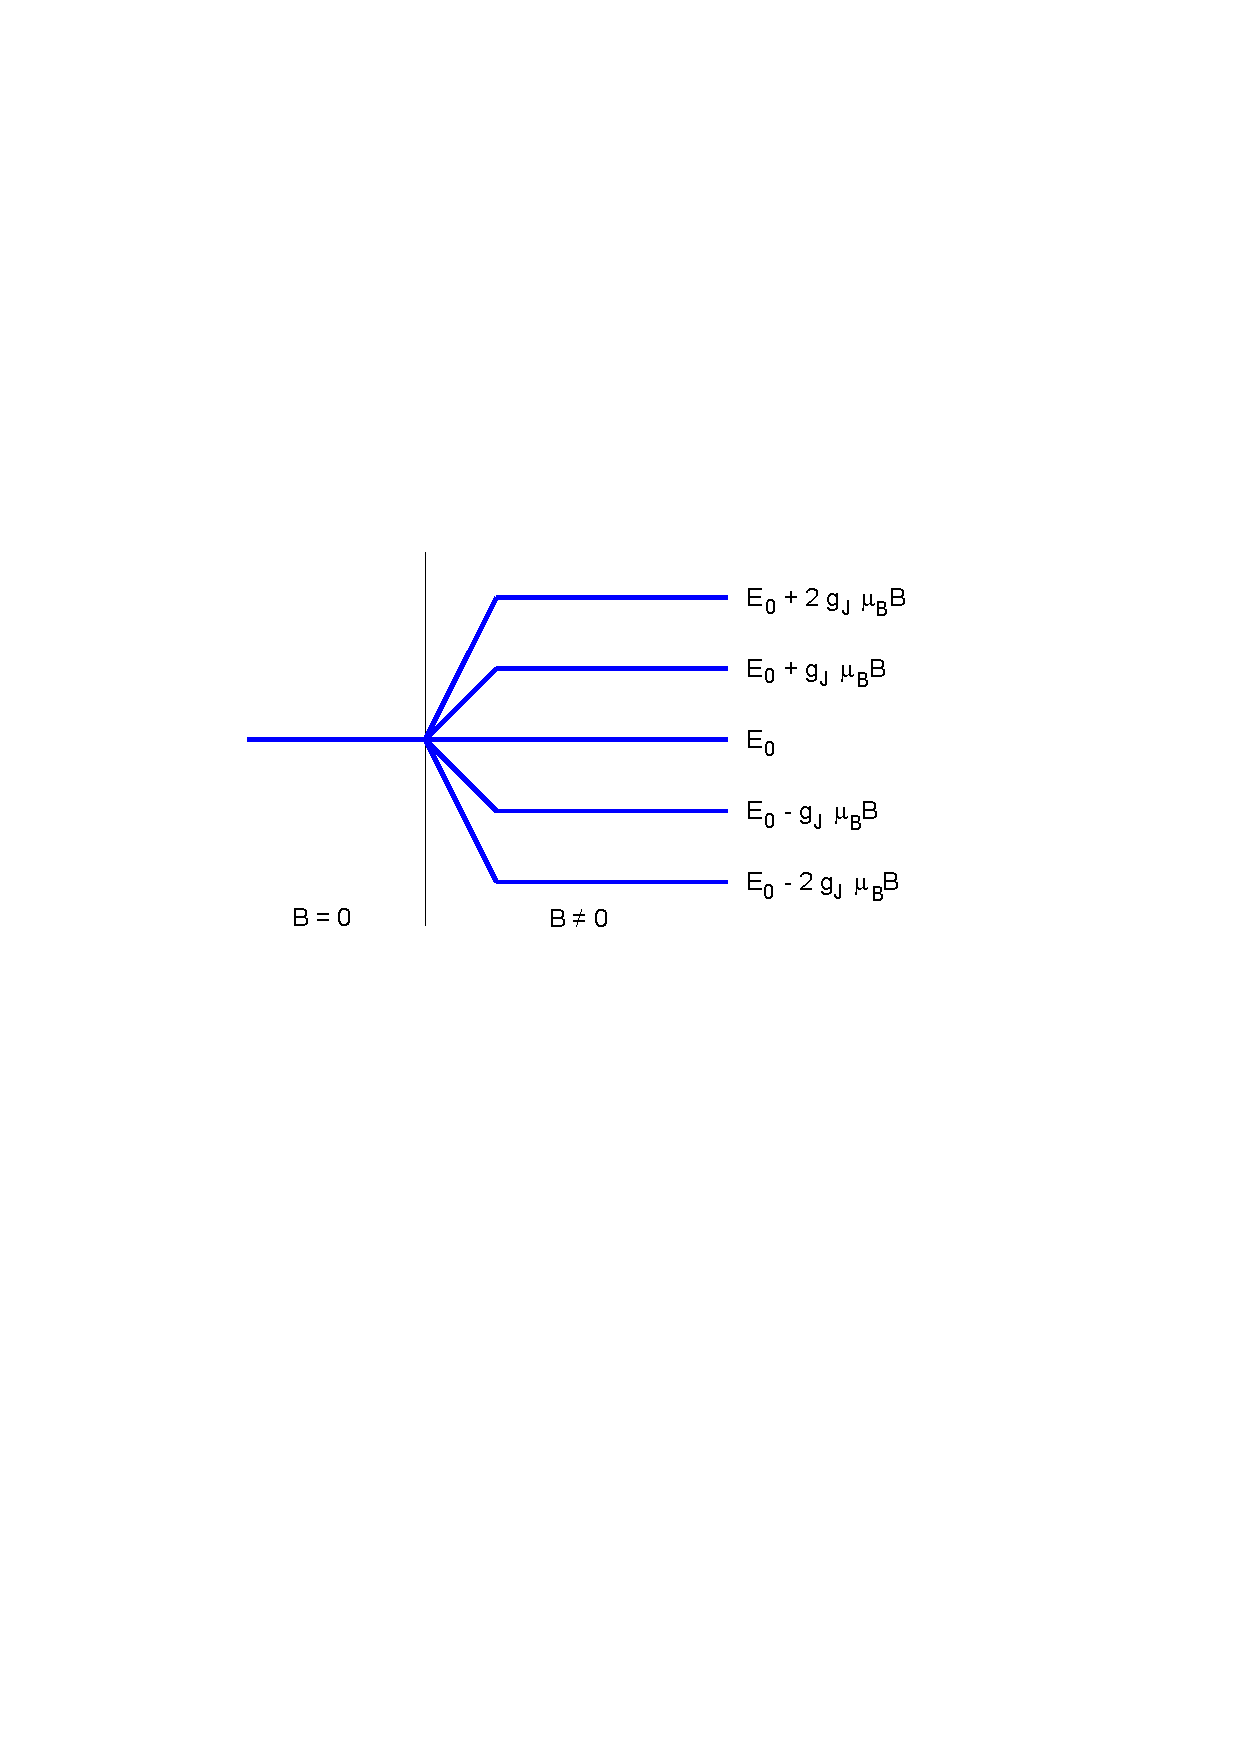
\includegraphics[width=0.6\textwidth]{graphics/aufspaltung.pdf}
    \caption{Schematische Darstellung der Aufspaltung eines Energieniveaus eines Atoms
    mit Gesamtdrehimpulsquantenzahl $J=2$.\cite{anleitung}}
    \label{fig:aufspaltung}
\end{figure}

\subsection{Auswahlregeln für Übergänge zwischen aufgespaltenen Energieniveaus}
\label{sec:auswahl}
Die Auswahlregeln sind für den Zeeman-Effekt sehr entscheidend, da sie festlegen welche
Übergänge zwischen verschiedenen Energieniveaus erlaubt sind.
Sie lassen sich durch die Betrachtung zweier möglicher Lösungen der zeitabhängigen
Schrödingergleichung mit den zugehörigen Energien $E_{\alpha}$ und $E_{\beta}$ bestimmen.
Die Linearkombination beider Zustände liefert einen Zustand, der eine Schwingung des
Elektrons mit der Frequenz
\begin{equation}
    \nu_{\alpha\beta}:=\frac{E_{\alpha}-E_{\beta}}{h}
\end{equation}
beschreibt.
Durch die Berechnung des elektrischen Dipolmomentes des Elektrons lässt sich die Intensität
der emittierten Strahlung bestimmen. Durch eine längere Rechnung lässt sich herleiten, dass
es nur zu einer Emission von Spektrallinien kommt, wenn sich die zu den Energien
gehörigen Orientierungsquantenzahlen $m_{\alpha}$ und $m_{\beta}$ entweder garnicht
oder um $\pm 1$ unterscheiden. Wobei es sich bei $\upD m=0$ um eine linear
polarisierte und parallel zum Magnetfeld emittierte Strahlung handelt und
ein Übergang mit $\upD m=\pm1$ zu einer zirkular polarisierten Strahlung führt.

\subsection{Der Zeeman-Effekt}

\subsubsection{Der normale Zeeman-Effekt}
Die oben gemachten Erkenntnisse gelten zunächst nur für $S=0$, da der Spin in der
zeitabhängigen Schrödingergleichung nicht auftaucht.
Daraus folgt mit Gleichung~\eqref{eq:g_J} immer $g_j=1$ unabhängig von $L$ und $J$.
Für die Energiedifferenz eines aufgespaltenen Niveaus ergibt sich aus
Gleichung~\eqref{eq:E_mag}
\begin{equation}
    \upD E=\upD m\mu_{\mathup{B}}B
    \label{eq:dE_norm}
\end{equation}
mit $\upD m=m_1-m_2$. Die möglichen Übergänge führen zu drei Liniengruppen mit
jeweils gleichem $\upD m$, dem sogenannten Zeeman-Triplett.
Abbildung~\ref{fig:zeeman_normal} zeigt die Aufspaltung und Übergänge für
$J=2\rightarrow J=1$.
Die linear polarisierten Linien mit $\upD m=0$ werden als $\pi$-Linien bezeichnet und sind nur
bei voller Intensität zu sehen, wenn sie senkrecht zur Feldrichtung betrachtet werden.
Somit ist das Aufspaltungsbild abhängig von der Beobachtungsrichtung.
Die zwei Liniengruppen mit $\upD m=\pm1$ werden als $\sigma$-Linien bezeichnet.
Die Liniengruppen selbst unterscheiden sich in ihrer Energie um jeweils den Wert
$\mu_{\mathup{B}}B$ voneinander.
\begin{figure}
    \centering
    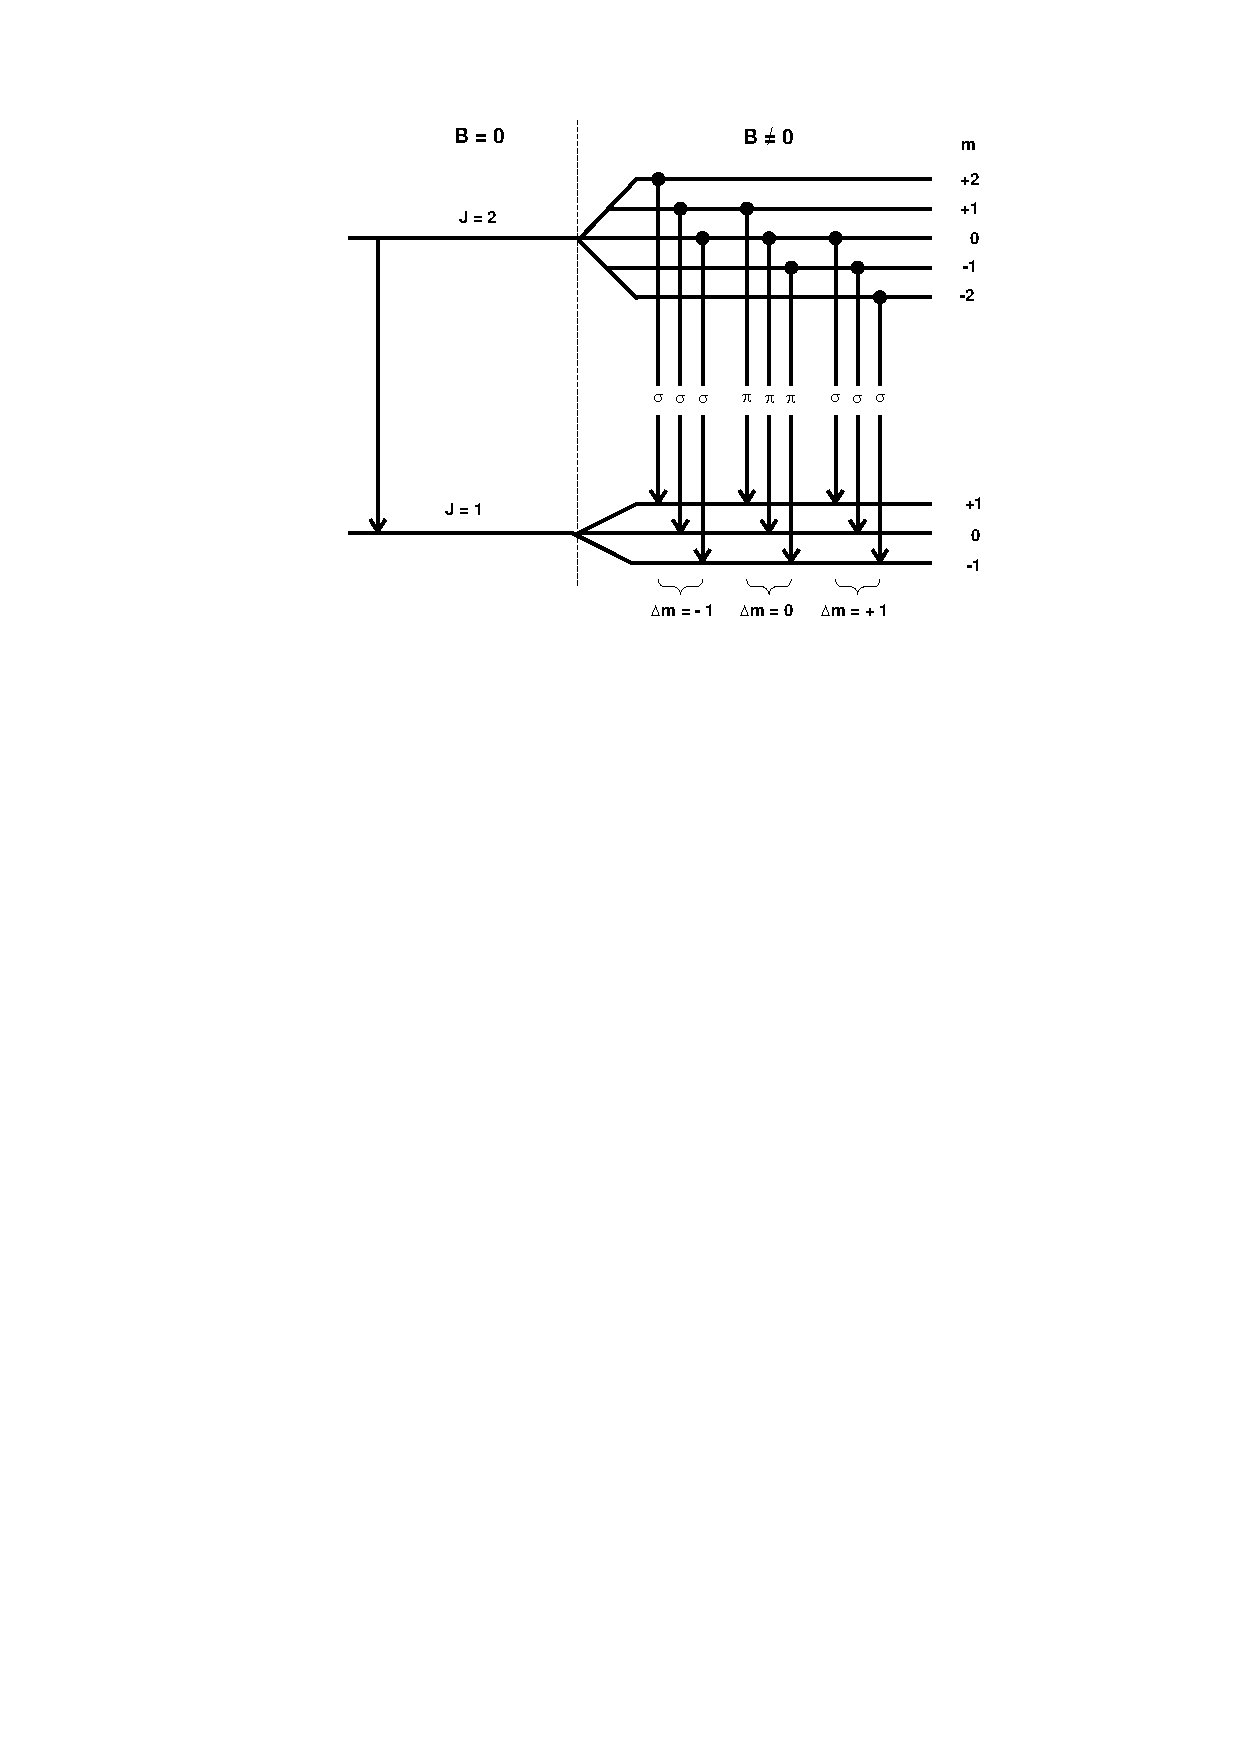
\includegraphics[width=0.65\textwidth]{graphics/zeeman_normal.pdf}
    \caption{Beispiel einer Linienaufspaltung beim normalen Zeeman-Effekt.\cite{anleitung}}
    \label{fig:zeeman_normal}
\end{figure}
Das der Spin $S=0$ ist, ist der natürlich seltener vorkommende Fall. Die Bezeichnung
normaler Zeeman-Effekt, lässt sich auf die frühere Entdeckung zurückführen.

\subsubsection{Der anomale Zeeman-Effekt}
Der häufiger anzutreffende anomale Zeeman-Effekt beschreibt den Fall $S\neq0$.
Tatsächlich führt die Herleitung der Auswahlregeln mit der spinabhängigen
Schrödingergleichung zu denselben Auswahlregeln wie in Abschnitt~\ref{sec:auswahl}.
Für die Energiedifferenz ergibt sich nun
\begin{equation}
    \upD E=\left[m_1g(L_1,S_1,J_1)-m_2g(L_2,S_2,J_2)\right]\mu_{\mathup{B}}B.
    \label{eq:dE_ano}
\end{equation}
Der Term in den eckigen Klammern stellt den Landé-Faktor des Übergangs dar.
Abbildung~\ref{fig:zeeman_anomal} zeigt beispielhaft die Aufspaltung und
Übergänge eines Alkali-Dubletts.
\begin{figure}
    \centering
    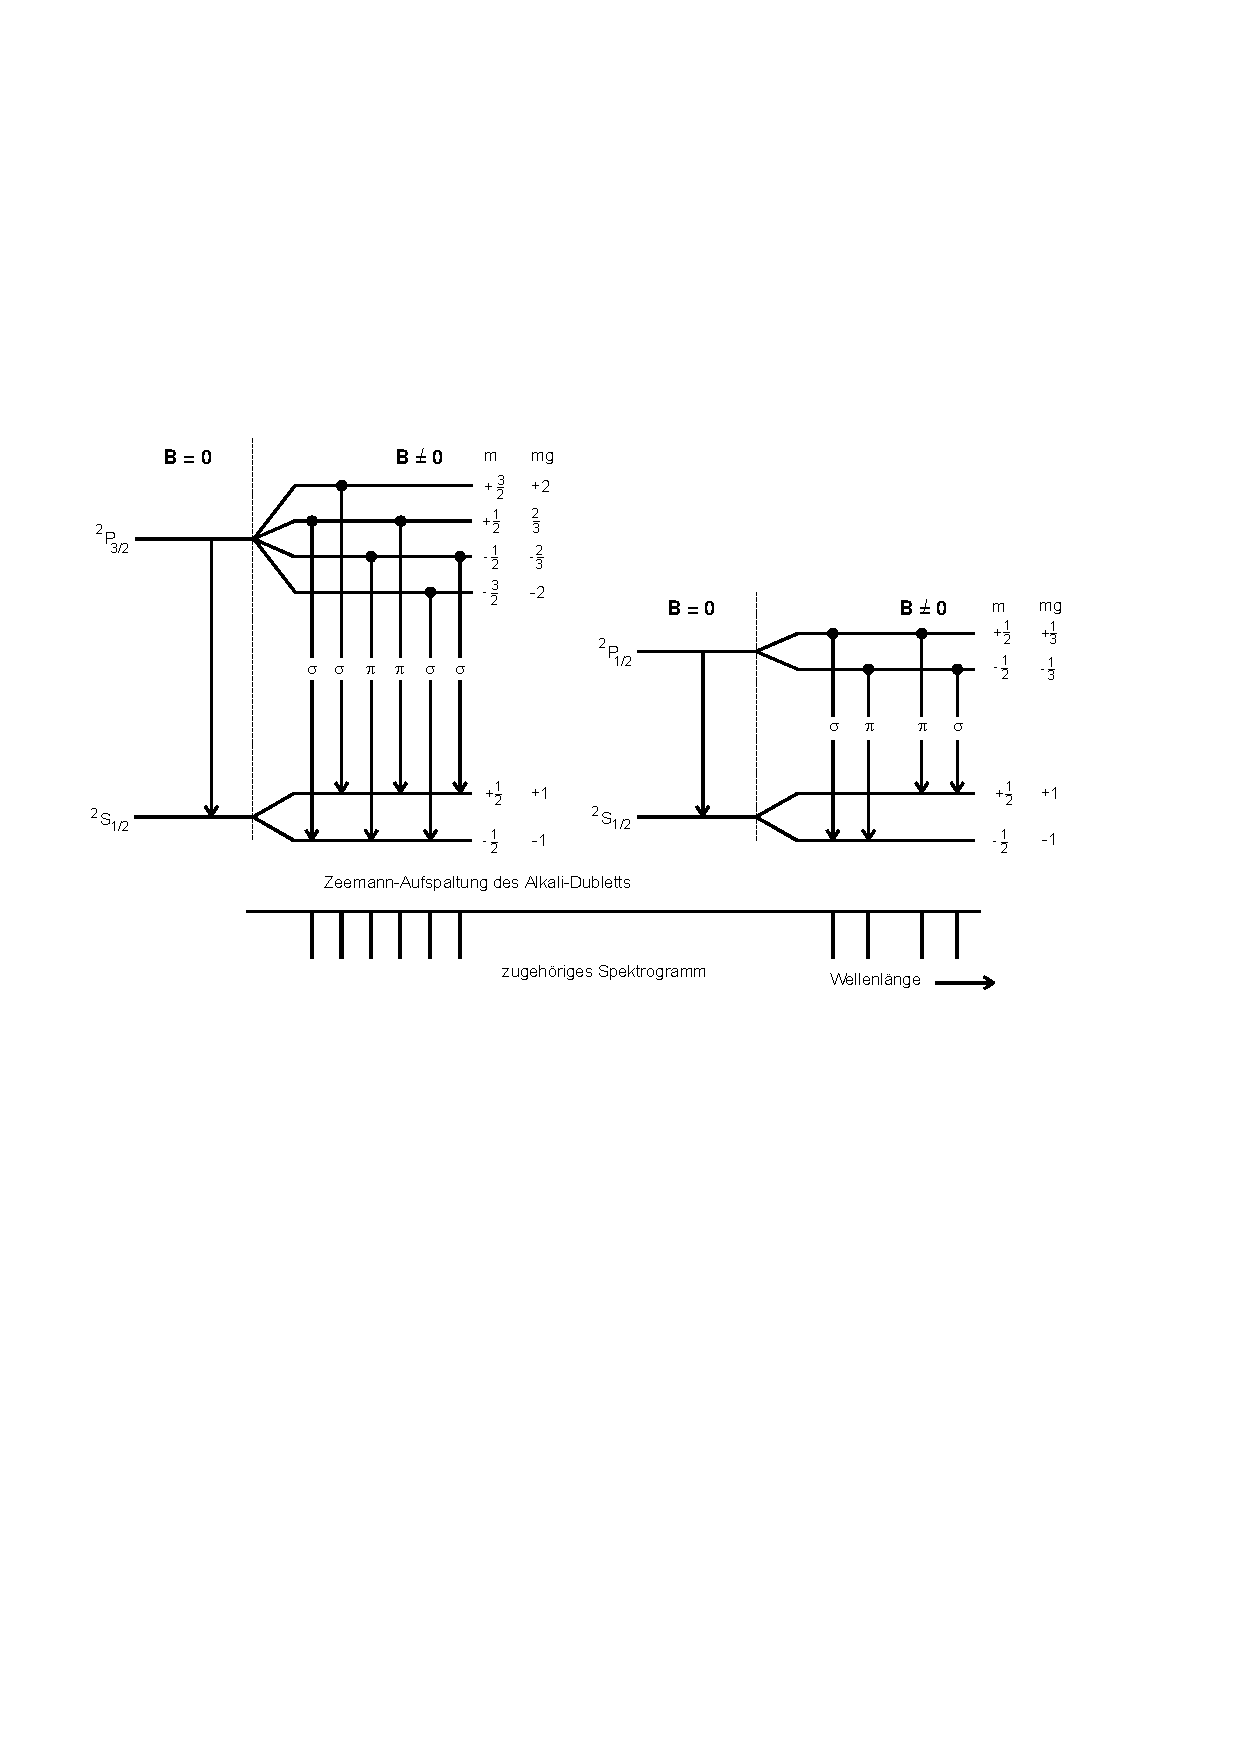
\includegraphics[width=\textwidth]{graphics/zeeman_anomal.pdf}
    \caption{Beispiel einer Linienaufspaltung beim anomalen Zeeman-Effekt.
    Dargestellt ist die Aufspaltung eines Alkali-Dubletts.\cite{anleitung}}
    \label{fig:zeeman_anomal}
\end{figure}

\section{Vorbereitung}
\label{sec:vorbereitung}
Vorbereitend zur Durchführung des Versuches sind im Folgenden die Energiedifferenzen
sowie die berechneten Landé-Faktoren für die zu untersuchenden Übergänge aufgeführt.

\subsection{Die rote Linie der Cd-Lampe}
Die Übergänge der Elektronen, welche die rote Linie erzeugen sind jene von~$^{1}D_2$
nach~$^{1}P_1$. Die zu den beiden Zuständen gehörenden Quantenzahlen sind in
Tabelle~\ref{tab:rot_cd} aufgeführt. Dort wird auch deutlich, dass es sich hierbei
um den normalen Zeeman-Effekt handelt, da beide Zustände den Spin $0$ besitzen. Der
Lande-Faktor ist hier für alle Zustände $g=1$. Mögliche Übergänge zwischen diesen
beiden Niveaus sind in Abbildung~\ref{fig:therm_rot} dargestellt. Die aus
Gleichung~\eqref{eq:dE_norm} bestimmten Energiedifferenzen der verschiedenen
Übergänge sind in Tabelle \ref{tab:rot_cdE} aufgeführt.
%
% \begin{figure}
%     \centering
%     \includegraphics[width=0.8\textwidth]{graphics/thermschema_rot.jpg}
%     \caption{Termschema der roten Linie.}
%     \label{fig:therm_rot}
% \end{figure}
%
\begin{table}[H]
    \centering
    \caption{Quantenzahlen der Übergänge.}
    \begin{tabular}{cccccc}
        \toprule
    {} & {$L$}  & {$J$}  & {$S$} & {$m$} & {$g$} \\
		\midrule
	  $^{1}D_2$ & 2 & 2 & 0 & $-2,-1,0,1,2$ & 1 \\
    $^{1}P_1$ & 1 & 1 & 0 & $-1,0,1$ & 1 \\
    \bottomrule
	\end{tabular}
    \label{tab:rot_cd}
\end{table}
%
\begin{table}[H]
    \centering
    \caption{Energieaufspaltung der Zeeman-Linien.}
    \begin{tabular}{cc}
        \toprule
    {Übergang} & {$\upD E$} \\
		\midrule
	  $\upD m=-1$ & $-\mu_{\mathup{B}}B$ \\
    $\upD m=0$ & 0 \\
    $\upD m=1$ & $\mu_{\mathup{B}}B$ \\
    \bottomrule
	\end{tabular}
    \label{tab:rot_cdE}
\end{table}
%
\subsection{Die blaue Linie der Cd-Lampe}
%
Die Übergänge der Elektronen, welche die blaue Linie erzeugen sind jene
von~$^{3}P_1$ nach~$^{3}S_1$. Die zu den beiden Zuständen gehörenden Quantenzahlen
sind in Tabelle~\ref{tab:blau_cd} aufgeführt. Die Zustände werden durch ein
anliegendes Magnetfeld aufgespalten. Durch die beiden gleich von Null verschiedenen
Spins wird auch deutlich, dass es sich hierbei um den anomalen Zeeman-Effekt handelt.
Der Lande-Faktor ist hier für alle Zustände $g\neq1$. Mögliche Übergänge zwischen
diesen beiden Niveaus sind in Abbildung~\ref{fig:therm_blau} dargestellt. Die aus
Gleichung~\eqref{eq:dE_ano} bestimmten Energiedifferenzen der verschiedenen Übergänge
sind in Tabelle \ref{tab:blau_cdE} aufgeführt.
%
% \begin{figure}
%     \centering
%     \includegraphics[width=0.8\textwidth]{graphics/thermschema_blau.jpg}
%     \caption{Termschema der blauen Linie.}
%     \label{fig:therm_blau}
% \end{figure}
%
\begin{table}[H]
    \centering
    \caption{Quantenzahlen der Übergänge.}
    \begin{tabular}{cccccc}
        \toprule
    {} & {$L$}  & {$J$}  & {$S$} & {$m$} & {$g$} \\
		\midrule
	  $^{3}P_1$ & 1 & 1 & 1 & $-1,0,1$ & 1,5 \\
    $^{3}S_1$ & 0 & 1 & 1 & $-1,0,1$ & 2 \\
    \bottomrule
	\end{tabular}
    \label{tab:blau_cd}
\end{table}
%
\begin{table}[H]
    \centering
    \caption{Energieaufspaltung der Zeeman-Linien.}
    \begin{tabular}{ccc}
        \toprule
    {Übergang} & {$m_1\rightarrow m_2$}  & {$\upD E$} \\
		\midrule
    \multirow{2}{*}{$\upD m=-1$}& 1\rightarrow 0 & $1,5\mu_{\mathup{B}}B$  \\
	   & 0\rightarrow -1  & $2\mu_{\mathup{B}}B$ \\ \hline
    \multirow{3}{*}{$\upD m=0$}& 1\rightarrow 1 & $-0,5\mu_{\mathup{B}}B$  \\
 	   & 0\rightarrow 0  & $0$ \\
     & -1\rightarrow-1 & $0,5\mu_{\mathup{B}}B$ \\ \hline
    \multirow{2}{*}{$\upD m=+1$}& 0\rightarrow 1 & $-2\mu_{\mathup{B}}B$  \\
 	   & -1\rightarrow 0  & $-1,5\mu_{\mathup{B}}B$ \\
    \bottomrule
	\end{tabular}
    \label{tab:blau_cdE}
\end{table}
%
\subsection{Zusammenfassung der Ergebnisse}
Zusammenfassend ergeben sich für die Übergänge der verschiedenen Linien die
in Tabelle~\ref{tab:lande} aufgeführten Ergebnisse für die Lande-Faktoren $|g|$.
Diese sollen im Versuch experimentell validiert werden.
%
\begin{table}[H]
    \centering
    \caption{Theoretische Vorhersage für $|g|$.}
    \begin{tabular}{ccc}
    \toprule
    {Linie} & {rot}  & {blau} \\
		\midrule
    $\sigma$ & 1 & 1,75  \\
	  $\pi$ & 0 & 0.5 \\
    \bottomrule
	\end{tabular}
    \label{tab:lande}
\end{table}
